\chapter{Premier principe de la thermodynamique}\label{chap:premierPrincipe}

\minitoc

\section*{Introduction}
\addcontentsline{toc}{section}{Introduction}

La thermodynamique est la discipline qui fait le lien entre les phénomènes mécaniques et thermiques.

Son but est de faire des bilans d'énergie sur des systèmes thermodynamiques au cours de transformations thermodynamiques.

\section{Transformations d'un système thermodynamique}

\subsection{Types de transformations}

Rappel : un système thermodynamique \(\paren{\Sigma}\) est à l'équilibre thermodynamique si ses paramètres d'état intensifs sont définis en tout point du système et ont la même valeur en tout instant.

Pour que \(\paren{\Sigma}\) évolue vers un autre état thermodynamique (\ie un autre état d'équilibre), il faut rompre le premier état d'équilibre en ajoutant ou en supprimant des contraintes.

Le passage d'un état d'équilibre à un autre est une transformation thermodynamique.

\subsubsection{Transformations infiniment lentes}

Au cours d'une transformation thermodynamique infiniment lente, le système passe par une succession d'états d'équilibre infiniment voisins les uns des autres.

Pour cela, il faut que le temps de réponse du système soit très faible, de sorte qu'après modification des contraintes, le système rejoigne un état d'équilibre.

Pour une transformation infiniment lente, \(\paren{\Sigma}\) est en état d'équilibre à tout instant.

\subsubsection{Transformations réversibles}

Il s'agit d'une transformation thermodynamique infiniment lente au cours de laquelle on peut inverser le sens de parcours.

Dans les deux sens, le système repasse par les mêmes états d'équilibre successifs.

Pour une transformation réversible, à tout instant, \(\paren{\Sigma}\) est en état d'équilibre et en équilibre avec le milieu extérieur.

\subsubsection{Transformations irréversibles}

Une transformation réversible est en réalité un modèle inatteignable.

Toute transformation est en réalité irréversible, soit parce qu'elle est rapide, soit parce qu'elle est lente mais non-renversable au cours du temps.

Les principales causes d'irréversibilité sont : \begin{itemize}
\item les transferts de matière et d'énergie dus aux hétérogénéités de température, de pression, de concentration, ... ;

\item les réactions chimiques en général ;

\item les frottements solides ou visqueux.\\
\end{itemize}

Par exemple, étudions la compression d'un gaz dans un cylindre.

\underline{Cas numéro 1 :}

\begin{tkz}[scale=1.5]
\draw (0,4.5) -- (0,0) -- (3,0) -- (3,4.5); % cylindre
\draw (0,3) -- (3,3); % haut piston
\draw (0,2.8) -- (3,2.8); % bas piston
\draw (1,3) -- (1,4) -- (2,4) -- (2,3); % masse
\foreach \i in {1,...,1000} \fill (rnd*3,rnd*2.8) circle (0.01); % atomes
\draw[->,red] (1.5,3.5) node[above,black] {\(m\)} -- (1.5,2.3) node[left] {\(\vec{P}\)}; % vecteur poids
\draw[<-] (2.7,2.9) -- (3.4,2.9) node[right] {piston mobile};
\draw[<-] (2.7, 0.3) -- (3.4,0.3) node[right] {gaz};
\end{tkz}

On dépose brutalement une masse \(m\) sur le piston mobile, qui descend donc rapidement, oscille, et finit par s'arrêter en raison des frottements.

La transformation n'est pas infiniment lente : juste après avoir déposé la masse, la pression et la température du gaz ne sont pas définies. La transformation est donc irréversible.

\underline{Cas numéro 2 :}

\begin{tkz}[scale=1.5]
\draw (0,4.5) -- (0,0) -- (3,0) -- (3,4.5); % cylindre
\draw (0,3) -- (3,3); % haut piston
\draw (0,2.8) -- (3,2.8); % bas piston
\foreach \i in {1,...,1000} \fill (rnd*3,rnd*2.8) circle (0.01); % atomes
\fill[pattern={Dots[distance=2pt]}] (1,3) -- (1.5,4) -- (2,3); % grains de sable
\draw[dotted] (1.5,4.6) -- (1.5,4); % grains de sable tombant
\draw[<-] (2.7,2.9) -- (3.4,2.9) node[right] {piston mobile};
\draw[<-] (2.7, 0.3) -- (3.4,0.3) node[right] {gaz};
\draw[<-] (1.55,4.3) -- (3.4,4.3) node[right,align=center] {on dépose des grains de sable doucement,\\jusqu'à obtenir la masse \(m\) sur le piston};
\end{tkz}

Le piston descend continûment, la transformation est infiniment lente, la température et la pression sont définies à tout instant. Le système est en équilibre avec le milieu extérieur. Donc la transformation est réversible.

Voyons un autre exemple, la détente d'un gaz :

\begin{tkz}
\draw (0,0) -- (3,0) -- (3,1) -- (6,1) -- (6,0) -- (9,0) -- (9,3) -- (6,3) -- (6,2) -- (3,2) -- (3,3) -- (0,3) -- (0,0); % contenant
\draw (4.5,2.5) -- (4.5,0.5); % robinet
\draw (4.4,2.5) -- (4.6,2.5); % robinet
\foreach \i in {1,...,142} \fill (3+rnd*1.5,1+rnd) circle (0.01); % gaz dans le couloir
\foreach \i in {1,...,858} \fill (3*rnd,3*rnd) circle (0.01); % gaz dans le carré
\draw[<-] (1.5,0.3) -- (1.5,-0.4) node[below] {gaz};
\draw[<-] (7.5,0.3) -- (7.5,-0.4) node[below] {\(\ensvide\)};
\end{tkz}

À \(t=0\), on ouvre le robinet :

\begin{tkz}
\draw (0,0) -- (3,0) -- (3,1) -- (6,1) -- (6,0) -- (9,0) -- (9,3) -- (6,3) -- (6,2) -- (3,2) -- (3,3) -- (0,3) -- (0,0); % contenant
\draw (4.5,4.5) -- (4.5,2.5); % robinet
\draw (4.4,4.5) -- (4.6,4.5); % robinet
\foreach \i in {1,...,160} \fill (3+rnd*3,1+rnd) circle (0.01); % gaz dans le couloir
\foreach \i in {1,...,420} \fill (3*rnd,3*rnd) circle (0.01); % gaz dans le carré de gauche
\foreach \i in {1,...,420} \fill (6+3*rnd,3*rnd) circle (0.01); % gaz dans le carré de droite
\end{tkz}

La transformation est irréversible : même en ouvrant le robinet doucement, la transformation est rapide. On n'a pas une succession d'états d'équilibre.

\subsubsection{Transformations particulières}

\(\begin{drcases}
T_{\paren{\Sigma}}=\cte&\text{transformation isotherme } \\
P_{\paren{\Sigma}}=\cte&\text{transformation isobare}
\end{drcases}\text{transformations réversibles}\)

\(\begin{drcases}
V_{\paren{\Sigma}}=\cte&\text{transformation isochore} \\
T_{\ext}=\cte&\text{transformation monotherme } \\
P_\ext=\cte&\text{transformation monobare}
\end{drcases}\text{transformations irréversibles}\)

\subsection{Énergie}

Rappel : dans un référentiel galiléen, on peut définir l'énergie interne \(U\) comme : \[U=E_{c_\text{micro}}+E_{p_\text{micro}}\] où \begin{description}
\item \(E_{c_\text{micro}}\) : la somme des énergies cinétiques microscopiques
\item \(E_{p_\text{micro}}\) : la somme des énergies potentielles microscopiques\\
\end{description} et l'énergie mécanique \(E_m\) comme : \[E_m=E_{c_\text{macro}}+E_{p_\text{macro}}\] avec \(E_{c_\text{macro}}=\dfrac{1}{2}m_{\paren{\Sigma}}v_{\paren{\Sigma}}^2\).

On définit alors l'énergie totale \(E\) comme : \[E=U+E_m.\]

C'est l'énergie totale stockée dans le système.

\subsection{Échanges d'énergie}

On reprend l'exemple du cylindre rempli de gaz avec un piston mobile :

\begin{tkz}[scale=1.5]
\draw (0,4.5) -- (0,0) -- (3,0) -- (3,4.5); % cylindre
\draw (0,3) -- (3,3); % haut piston
\draw (0,2.8) -- (3,2.8); % bas piston
\draw (1,3) -- (1,4) -- (2,4) -- (2,3); % masse
\foreach \i in {1,...,1000} \fill (rnd*3,rnd*2.8) circle (0.01); % atomes
\draw[->,red] (1.5,3.5) node[above,black] {\(m\)} -- (1.5,2.3) node[left] {\(\vec{P}\)}; % vecteur poids
\draw[<-] (2.7,2.9) -- (3.4,2.9) node[right] {piston mobile};
\draw[<-] (2.7, 0.3) -- (3.4,0.3) node[right] {gaz};
\end{tkz}

Si on pose une masse \(m\) sur le piston mobile, celui-ci s'enfonce. Donc la masse a cédé une partie de son énergie potentielle au système.

Expérimentalement, on remarque que si la température augmente, l'énergie interne augmente.

Il y a eu transfert d'énergie entre le travail du poids et l'énergie interne du système.

On plonge le cylindre dans une eau chaude :

\begin{tkz}[scale=1.5]
\draw (0,6.5) -- (0,0) -- (6,0) -- (6,6.5); % bac
\draw (0,4) -- (2,4); % eau
\draw (5,4) -- (6,4); % eau
\draw (2,6) -- (2,1.5) -- (5,1.5) -- (5,6); % cylindre
\draw (2,4.5) -- (5,4.5); % haut piston
\draw (2,4.3) -- (5,4.3); % bas piston
\foreach \i in {1,...,1000} \fill (2+rnd*3,1.5+rnd*2.8) circle (0.01); % atomes
\draw[<-] (4.7,4.4) -- (6.4,4.4) node[right] {piston mobile};
\draw[<-] (4.7, 1.8) -- (6.4,1.8) node[right] {gaz};
\draw[->] (-0.4,0.3) node[left] {eau chaude} -- (0.3,0.3);
\end{tkz}

Alors, la température du gaz augmente et donc son énergie interne aussi.

Il y a eu transfert d'énergie entre l'eau et le gaz.

Le transfert d'énergie sans transfert de matière ni déplacement s'appelle le transfert thermique \(Q\).

Le transfert thermique s'interprète au niveau microscopique comme l'agitation thermique se propageant de proche en proche à travers le cylindre.

On a le tableau suivant :

\begin{center}
\begin{tabular}{|l|c|c|}
\hline
\diagbox{Grandeur\\énergétique}{Échelle} & Macroscopique & Microscopique \\
\hline
Énergie & \(E_m\) & \(U\) \\
\hline
Transfert d'énergie & \(W\) & \(Q\) \\
\hline
\end{tabular}
\end{center}

\section{Premier principe de la thermodynamique}

\subsection{Énoncé}

Pour tout système fermé \(\paren{\Sigma}\), on peut définir une fonction \(U\) dépendant des variables d'état extensives et telle que l'énergie totale du système \(E=E_m+U\) soit conservative, c'est-à-dire se conserve si \(\paren{\Sigma}\) est isolé. \(U\) est l'énergie interne du système.

C'est un principe de conservation. Il traduit l'impossibilité de création d'énergie.

\subsection{Bilan d'énergie}

Si l'on fait un bilan d'énergie sur \(\paren{\Sigma}\), on obtient : \[\adif{E}=\adif{\paren{E_m+U}}=W+Q.\]

Si \(\paren{\Sigma}\) est au repos (\(E_{c_\text{macro}}=\cte\) et \(E_{p_\text{macro}}=\cte\)) alors \(\adif{E_m}=0\) donc : \[\adif{U}=W+Q.\] C'est la forme réduite du premier principe de la thermodynamique (Carnot, 1850). Cette expression donne l'équivalence travail/transfert thermique (Joule).

On peut donc faire varier \(U\) à l'aide soit d'un travail \(W\), soit d'un transfert thermique \(Q\).

Pour un système en évolution cyclique, les états d'équilibre initiaux et finaux sont égaux. Donc : \[\adif{U}=0.\]

Convention : \(W\) et \(Q\) sont toujours orientés vers le système.

Si \(Q>0\) ou \(W>0\), \(U\) augmente car le système reçoit du travail ou du transfert thermique du milieu extérieur.

Si \(Q<0\) ou \(W<0\), \(U\) diminue car le système fournit du travail ou du transfert thermique au milieu extérieur.

\section{Travail des forces de pression}

\subsection{Expression générale}

On considère un fluide \(\Sigma\) dans un cylindre avec un piston mobile de surface \(S\) :

\begin{tkz}[scale=1.8]
\draw[->] (-1,0) -- (4.5,0) node[below right] {\(x\)}; % axe
\draw[->,blue,thick] (0,0) -- (1,0) node[below right] {\(\vec{u}_x\)}; % vecteur unitaire ux
\draw (0,0.1) -- (0,-0.1) node[below] {\(O\)}; % graduation O
\draw (2,0.1) -- (2,-0.1) node[below] {\(x\)}; % graduation x
\draw (2.8,0.1) -- (2.8,-0.1) node[below] {\(x+\odif{x}\)}; % graduation x+dx
\draw (3.5,3) -- (0,3) -- (0,1) node[above right] {\(\Sigma\)} -- (3.5,1); % cylindre
\draw (2,3) -- (2,1); % piston gauche
\draw (2.8,3) -- (2.8,1); % piston droit
\draw[<->] (1.9,3) -- (1.9,1) node[left,pos=0.5] {\(S\)}; % surface S
\draw[<->] (2,3.1) -- (2.8,3.1) node[above,pos=0.5] {\(\odif{x}\)}; % distance dx
\fill[pattern=north east lines] (2,3) -- (2.8,3) -- (2.8,1) -- (2,1); % volume dV
\draw[<-] (2.5,2.7) -- (3.8,2.7) node[right] {\(\odif{V}\)};
\node at (3.4,1.5) {\(P_\ext\)};
\draw[<-] (2,1) -- (2.4,0.6);
\draw[<-] (2.8,1) -- (2.4,0.6) node[below] {piston mobile};
\end{tkz}

On exerce une contrainte (\(P_\ext\)) sur le piston. Si la transformation de \(\Sigma\) est quelconque, la pression \(P\) et la température \(T\) du fluide ne sont pas forcément définies. La pression extérieure l'est toujours.

Le piston se déplace de \(\odif{x}\) donc on a un accroissement du volume de \(\Sigma\) de : \[\odif{V}=S\odif{x}.\]

Ainsi, on a la force pressante \(\vec{F}\) exercée par le milieu extérieur sur \(\Sigma\) : \[\vec{F}=-SP_\ext\vec{u}_x.\]

D'où le travail élémentaire : \[\fdif{W}=\vec{F}\scal\odif{\vec{l}}=-SP_\ext\odif{x}=-P_\ext\odif{V}.\]

\(\fdif{W}\) est algébrique : \(\fdif{W}\supinf0\).

Si \(\odif{V}<0\) (compression) alors \(\fdif{W}>0\) : le système reçoit du travail du milieu extérieur.

Si \(\odif{V}>0\) (détente) alors \(\fdif{W}<0\) : le système fournit du travail au milieu extérieur.

Au cours d'une transformation non-élémentaire, on a le travail : \[W=\int\fdif{W}=\int_{V_1}^{V_2}-P_\ext\odif{V}=-\int_{V_1}^{V_2}P_\ext\odif{V}.\]

Donc on a une formule pour calculer le travail des forces de pression.

Si la transformation est réversible, \(\Sigma\) est en équilibre avec le milieu extérieur donc \(P=P_\ext\). On a donc : \[W=-\int_{V_1}^{V_2}P\odif{V}.\]

On a besoin de \(P\paren{V}\) pour obtenir l'équation d'état.

\subsection{Transformations usuelles}

\subsubsection{Transformation isochore}

On a \(V=\cte\) donc \(\odif{V}=0\) donc : \[W=0.\]

\subsubsection{Transformation monobare}

On a \(P_\ext=\cte\) donc : \[W=-P_\ext\int_{V_1}^{V_2}\odif{V}=-P_\ext\paren{V_2-V_1}.\]

\subsubsection{Transformation isobare}

On a \(P=P_\ext=\cte\) donc : \[W=-P\paren{V_2-V_1}.\]

\subsubsection{Transformation isotherme}

On a \(T=\cte\) et \(P=P_\ext\) donc : \[W=-\int_{V_1}^{V_2}P\odif{V}.\]

Si on a un gaz parfait, on a \(PV=nRT\) donc : \[P=\dfrac{nRT}{V}.\]

Donc on a : \[W=-\int_{V_1}^{V_2}\dfrac{nRT}{V}\odif{V}=-nRT\ln\paren{\dfrac{V_2}{V_1}}.\]

\subsection{Représentation graphique}

Dans le cas d'une transformation réversible, on a \(W=-\int_{V_1}^{V_2}P\odif{V}\).

Donc le travail est l'aire sous la courbe \(P\paren{V}\) :

\begin{tkz}
\begin{axis}[axis lines=left,
xlabel={\(V\)},
ylabel={\(P\)},
xmin=0,xmax=6,
ymin=0,ymax=2.5,
xtick={1,4},
xticklabels={\(V_1\),\(V_2\)},
ytick={0},
xlabel style={at={(axis description cs:1,0)},anchor=north west},
ylabel style={at={(axis description cs:0,1)},anchor=south east,rotate=-90}]
\addplot[name path=A,domain=1:4,samples=1000] {exp(-x)+1};
\addplot[domain=0:6,samples=1000] {exp(-x)+1};
\addplot[name path=B,domain=1:4,samples=1000] {0};
\addplot[pattern={Lines[angle=45,distance=3mm]}] fill between [of=A and B];
\end{axis}
\end{tkz}

Un tel diagramme est appelé diagramme de Watt. On a \(\abs{W}=\begin{tikzpicture}
\filldraw[pattern={Lines[angle=45,distance=3mm]}] (0,-0.25) -- (0,0.25) -- (1,0.25) -- (1,-0.25) -- (0,-0.25);
\end{tikzpicture}\)

\subsubsection{Transformation isobare}

On a \(P=\cte\) :

\begin{tkz}
\begin{axis}[axis lines=left,
xlabel={\(V\)},
ylabel={\(P\)},
xmin=0,xmax=6,
ymin=0,ymax=2.5,
xtick={1,4},
xticklabels={\(V_1\),\(V_2\)},
ytick={0},
xlabel style={at={(axis description cs:1,0)},anchor=north west},
ylabel style={at={(axis description cs:0,1)},anchor=south east,rotate=-90}]
\addplot[name path=A,domain=1:4,samples=1000] {2};
\addplot[domain=0:6,samples=1000] {2};
\addplot[name path=B,domain=1:4,samples=1000] {0};
\addplot[pattern={Lines[angle=45,distance=3mm]}] fill between [of=A and B];
\end{axis}
\end{tkz}

On a \(W=-P\paren{V_2-V_1}=-\,\begin{tikzpicture}
\filldraw[pattern={Lines[angle=45,distance=3mm]}] (0,-0.25) -- (0,0.25) -- (1,0.25) -- (1,-0.25) -- (0,-0.25);
\end{tikzpicture}\)

\subsubsection{Évolution cyclique}

\begin{tkz}
\begin{axis}[axis lines=left,
xlabel={\(V\)},
ylabel={\(P\)},
xmin=0,xmax=6,
ymin=0,ymax=3,
xtick={1,5},
xticklabels={\(V_1\),\(V_2\)},
ytick={0},
xlabel style={at={(axis description cs:1,0)},anchor=north west},
ylabel style={at={(axis description cs:0,1)},anchor=south east,rotate=-90},
trig format plots=rad]
%\draw (axis cs:3,1.5) ellipse (2 and 0.8);
\addplot[name path=A,domain=0:pi,samples=1000] ({3+2*cos(x)},{1.5+0.8*sin(x)});
\addplot[name path=C,domain=pi:2*pi,samples=1000] ({3+2*cos(x)},{1.5+0.8*sin(x)});
\addplot[name path=B,domain=1:5,samples=1000] {0};
\addplot[pattern={Lines[angle=-45,distance=3mm]},pattern color=blue] fill between [of=A and B];
\addplot[pattern={Lines[angle=45,distance=3mm]},pattern color=red] fill between [of=C and B];
\addplot[pattern={Lines[angle=90,distance=3mm]}] fill between [of=C and A];
\addplot[domain=0:2*pi,samples=1000,decoration={markings,mark=at position 0.25 with {\arrow{<}},mark=at position 0.75 with {\arrow{<}}},postaction={decorate},very thick] ({3+2*cos(x)},{1.5+0.8*sin(x)});
\end{axis}
\end{tkz}

De \(V_1\) à \(V_2\) on a : \[W_\text{aller}=-\int_{V_1}^{V_{2}}P\odif{V}=-\,\begin{tikzpicture}
\filldraw[pattern={Lines[angle=-45,distance=3mm]},pattern color=blue] (0,-0.25) -- (0,0.25) -- (1,0.25) -- (1,-0.25) -- (0,-0.25);
\end{tikzpicture}\]

De \(V_2\) à \(V_1\) on a : \[W_\text{retour}=-\int_{V_2}^{V_{1}}P\odif{V}=\begin{tikzpicture}
\filldraw[pattern={Lines[angle=45,distance=3mm]},pattern color=red] (0,-0.25) -- (0,0.25) -- (1,0.25) -- (1,-0.25) -- (0,-0.25);
\end{tikzpicture}\]

Donc on a : \[W_\text{cycle}=W_\text{aller}+W_\text{retour}=-\,\begin{tikzpicture}
\filldraw[pattern={Lines[angle=90,distance=3mm]}] (0,-0.25) -- (0,0.25) -- (1,0.25) -- (1,-0.25) -- (0,-0.25);
\end{tikzpicture}\] donc : \[\abs{W_\text{cycle}}=A_\text{cycle}\] où \(A_\text{cycle}\) désigne l'aire du cycle.

Si on a un cycle dans ce sens : \begin{tikzpicture}
\draw[decoration={markings,mark=at position 1 with {\arrow{<}}},postaction={decorate}] (0,0) circle (0.5);
\end{tikzpicture} alors le système est moteur : il fournit du travail au milieu extérieur.

Si on a un cycle dans ce sens : \begin{tikzpicture}
\draw[decoration={markings,mark=at position 1 with {\arrow{>}}},postaction={decorate}] (0,0) circle (0.5);
\end{tikzpicture} alors le système est récepteur : il reçoit du travail du milieu extérieur.

Le travail dépend du chemin suivi (il n'est donc pas conservatif) :

\begin{tkz}
\begin{axis}[axis lines=left,
xlabel={\(V\)},
ylabel={\(P\)},
xmin=0,xmax=6,
ymin=0,ymax=2.5,
ytick={0},
xmajorticks=false,
xlabel style={at={(axis description cs:1,0)},anchor=north west},
ylabel style={at={(axis description cs:0,1)},anchor=south east,rotate=-90}]
\fill[pattern={Lines[angle=45,distance=3mm]},pattern color=blue] (1,2) -- (4,2) -- (4,0) -- (1,0) -- (1,2);
\fill[pattern={Lines[angle=-45,distance=3mm]},pattern color=red] (1,2) -- (4,1) -- (4,0) -- (1,0) -- (1,2);
\addplot[name path=A,samples=1000,blue,ultra thick,decoration={markings,mark=at position 0.5 with {\arrow{>}}},postaction={decorate}] coordinates {(1,2) (4,2) (4,1)};
\addplot[name path=C,samples=1000,red,ultra thick,decoration={markings,mark=at position 0.5 with {\arrow{>}}},postaction={decorate}] coordinates {(1,2) (4,1)};
\end{axis}
\end{tkz}

On a bien \(\begin{tikzpicture}
\filldraw[pattern={Lines[angle=-45,distance=3mm]},pattern color=red] (0,-0.25) -- (0,0.25) -- (1,0.25) -- (1,-0.25) -- (0,-0.25);
\end{tikzpicture}\,\not=\,\begin{tikzpicture}
\filldraw[pattern={Lines[angle=45,distance=3mm]},pattern color=blue] (0,-0.25) -- (0,0.25) -- (1,0.25) -- (1,-0.25) -- (0,-0.25);
\end{tikzpicture}\)

\section{Transferts thermiques}

\subsection{Méthode de calcul}

D'après le premier principe de la thermodynamique, on a \(\adif{U}=W+Q\) donc on a : \[Q=\adif{U}-W.\] On doit calculer \(\adif{U}\) et \(W\) pour calculer \(Q\).

\subsection{Transformations particulières}

\subsubsection{Transformation isochore}

On a \(V=\cte\) donc \(W=0\) donc \[Q_V=\adif{U}.\]

\subsubsection{Transformation monobare}

On a \(P_\ext=\cte\) donc \(W=-P_\ext\paren{V_2-V_1}\) donc on a : \[\begin{aligned}
Q&=\adif{U}-W \\
&=U_2-U_1+P_\ext\paren{V_2-V_1} \\
&=U_2+P_\ext V_2-\paren{U_1+P_\ext V_1}.
\end{aligned}\]

On pose \(H^*=U+P_\ext V\) et on a donc : \[Q=H_2^*-H_1^*.\]

\(H^*\) est en fonction de \(P_\ext\) donc ce n'est pas une fonction d'état.

On impose donc une nouvelle contrainte : le système doit être en équilibre avec le milieu extérieur aux états initial et final. Ainsi, à l'état initial on a \(P_1=P_\ext\), et à l'état final on a \(P_2=P_\ext\).

On définit donc la fonction d'état appelée enthalpie par : \[H=U+PV.\]

Ainsi, pour une transformation monobare entre états d'équilibre, on a : \[Q=H_2-H_1=\adif{H}.\]

\subsection{Capacités thermiques}

On travaille avec un corps pur monophasé soumis aux seules forces de pression.

Les paramètres d'état \(T\), \(P\) et \(V\) sont liés par une équation d'état. Seuls deux suffisent pour décrire le système.

\subsubsection{Choix du couple \(\paren{T,V}\) (variables naturelles de \(U\))}

On a : \[\begin{WithArrows}
U&=U\paren{T,V} \Arrow{\(\dif\)} \\
\odif{U}&=\pdv{U}{T}_V\odif{T}+\pdv{U}{V}_T\odif{V}.
\end{WithArrows}\]

On définit la capacité thermique à volume constant (en \(\unit{\joule\per\kelvin}\)) par : \[C_V=\pdv{U}{T}_V\]

On considère une transformation isochore. On a donc \(Q_V=\adif{U}\) d'après le premier principe de la thermodynamique.

De plus, on a \(\odif{U}=C_V\odif{T}+0\) donc : \[\adif{U}=\int_{T_1}^{T_2}C_V\odif{T}.\]

Enfin, si \(C_V=\cte\) alors on a : \[\adif{U}=C_V\paren{T_2-T_1}.\]

\(C_V\) est donnée par les tables thermodynamiques.

On peut donc calculer \(\adif{U}\) et \(Q\) à partir des températures \(T_1\) et \(T_2\).

\subsubsection{Choix du couple \(\paren{T,P}\) (variables naturelles de \(H\))}

On a : \[\begin{WithArrows}
H&=H\paren{T,P} \Arrow{\(\dif\)} \\
\odif{H}&=\pdv{H}{T}_{P}\odif{T}+\pdv{H}{P}_{T}\odif{P}.
\end{WithArrows}\]

On définit la capacité thermique à pression constante (en \(\unit{\joule\per\kelvin}\)) par : \[C_P=\pdv{H}{T}_P\]

On définit aussi les capacités thermiques à pression constante molaire et massique par : \[C_{P_m}=\dfrac{C_P}{n}\quad\text{et}\quad c_P=\dfrac{C_P}{m}.\]

On a : \[\begin{WithArrows}
H&=U+PV \Arrow[i]{\(\dif\)} \\
\odif{H}&=\odif{U}+\odif{\paren{PV}} \\
&=\odif{U}+V\odif{P}+P\odif{V} \\
&=\fdif{W}+\fdif{Q}+V\odif{P}+P\odif{V}.
\end{WithArrows}\]

On considère une transformation isobare. On a donc \(P_\ext=P=\cte\). On a donc : \[\fdif{W}=-P_\ext\odif{V}=-P\odif{V}.\] Donc on a : \[\begin{WithArrows}
\odif{H}&=\fdif{Q} \Arrow{\(\textstyle\int\)} \\
\adif{H}&=Q_P.
\end{WithArrows}\]

On a aussi : \[\begin{WithArrows}
\odif{H}&=C_P\odif{T} \Arrow{\(\textstyle\int\)} \\
\adif{H}&=\int_{T_1}^{T_2}C_P\odif{T}.
\end{WithArrows}\]

Enfin, si \(C_P=\cte\), on a : \[\adif{H}=C_P\paren{T_2-T_1}.\]

\(C_P\) est donnée par les tables thermodynamiques.

On peut donc calculer \(\adif{H}\) à partir des températures \(T_1\) et \(T_2\).

Par exemple, calculons la variation d'enthalpie associée au passage d'un mélange gazeux de la température \(T_1=\SI{298}{\kelvin}\) à \(T_2=\SI{600}{\kelvin}\). On a \(C_{P_m}=\paren{\num{31.4}+\num{2.1e-2}T}\unit{\joule\per\kelvin\per\mole}\) (valable sur \(\intervii{T_1}{T_2}\)). On a \(n=\SI{1}{\mole}\). On a donc : \[\begin{aligned}
\adif{H}&=\int_{T_1}^{T_2}C_P\odif{T} \\
&=\int_{T_1}^{T_2}nC_{P_m}\odif{T} \\
&=\int_{T_1}^{T_2}\paren{\num{31.4}+\num{2.1e-2}T}\odif{T} \\
&=\croch{\num{31.4}T+\dfrac{\num{2.1e-2}}{2}T^2}_{T_1}^{T_2} \\
&=\SI{12.3}{\kilo\joule}
\end{aligned}\]

Pour un gaz parfait, on a : \[\begin{WithArrows}
H&=U+PV \Arrow{\(\pdv{}{T}\)} \\
\pdv{H}{T}_P&=\pdv{U}{T}_V+\pdv{\paren{PV}}{T}_{P\text{ ou }V} \\
\pdv{H}{T}_P&=\pdv{U}{T}_V+\pdv{\paren{nRT}}{T}_{P\text{ ou }V} \\
C_P&=C_V+nR.
\end{WithArrows}\]

On en déduit les relations : \[C_{P_m}=C_{V_m}+R\] et \[\begin{aligned}
c_P&=c_V+\dfrac{n}{m}R \\
&=c_V+\dfrac{R}{M}
\end{aligned}\] où \(M\) est la masse molaire du gaz considéré.

On a donc les relations de Mayer pour les gaz parfaits : \[C_P=C_V+nR\qquad C_{P_m}=C_{V_m}+R\qquad c_P=c_V+\dfrac{R}{M}.\]

On définit l'indice adiabatique (sans unité) par : \[\gamma=\dfrac{C_P}{C_V}.\]

On obtient deux relations (uniquement valables pour les gaz parfaits) : \[C_{P_m}=\dfrac{\gamma R}{\gamma-1}\quad\text{et}\quad C_{V_m}=\dfrac{R}{\gamma-1}.\]

Par exemple : \begin{itemize}
\item pour un gaz parfait monoatomique, on a \(C_{V_m}=\dfrac{3}{2}R\) et \(C_{P_m}=\dfrac{5}{2}R\) donc \(\gamma=\dfrac{5}{3}=\num{1.67}\) ;
\item pour un gaz parfait diatomique, on a \(C_{V_m}=\dfrac{5}{2}R\) et \(C_{P_m}=\dfrac{7}{2}R\) donc \(\gamma=\dfrac{7}{5}=\num{1.4}\) ;
\item pour l'air ambiant, on mesure \(\gamma=\num{1.41}\) ce qui confirme la large majorité du dioxygène et du diazote dans sa composition. \\
\end{itemize}

Pour les phases condensées, \ie indilatables et incompressibles, quelles que soient la température et la pression, on a \(V=\cte\). Donc dans les conditions normales de température et de pression, on a : \[H=U\] et la capacité thermique (en \(\unit{\joule\per\kelvin}\)) : \[C=C_V=C_P.\]

Si \(C\) est une constante dans l'intervalle de températures considéré alors on a : \[\adif{H}=\adif{U}=C\adif{T}=Q\] car \(\adif{U}=W+Q\) avec \(W=-\int P_\ext\odif{V}=0\).

Ordres de grandeur : \begin{itemize}
\item on a \(C_\text{eau}=\SI{4.185}{\kilo\joule\per\kelvin\per\kilo\gram}=\SI{1}{\cal\per\kelvin\per\gram}\), avec \(\SI{1}{\cal}=\SI{4.185}{\joule}\) (une calorie est l'énergie qu'il faut fournir à \(\SI{1}{\gram}\) d'eau pour élever sa température de \(\SI{1}{\kelvin}\) ou de \(\SI{15}{\degreeCelsius}\) à \(\SI{16}{\degreeCelsius}\)) ;
\item on a \(C_\text{fer}=\SI{0.46}{\kilo\joule\per\kelvin\per\kilo\gram}\approx\num{0.1}C_\text{eau}\).
\end{itemize}

\section{Transformation adiabatique d'un gaz parfait}

\subsection{Transformation réversible}

On passe d'un état initial avec une pression \(P_1\), une température \(T_1\) et un volume \(V_1\) à un état final avec une pression \(P_2\), une température \(T_2\) et un volume \(V_2\) par le biais d'une transformation adiabatique (donc \(Q=0\) et \(T\not=T_\ext\)) et réversible (donc \(P=P_\ext\not=\cte\)) :

\begin{tkz}[scale=1.6]
\filldraw[pattern={Lines[angle=-45,distance=5mm]}] (0,0) -- (5,0) -- (5,4) -- (4,4) -- (4,1) node[above left] {\(\Sigma\)} -- (1,1) node[above right] {\(P,T,V\)} -- (1,4) -- (0,4) -- (0,0); % enceinte isolée
\filldraw[pattern={Lines[angle=-45,distance=5mm]}] (1,3.5) -- (4,3.5) -- (4,3.3) -- (1,3.3) -- (1,3.5); % piston isolé
\node at (2.5,4.2) {\(P_\ext\)};
\draw[<-] (3.7,3.4) -- (5.4,3.4) node[right] {piston mobile (\(P=P_\ext\))};
\draw[<-] (4.7,0.3) -- (5.4,0.3) node[right] {enceinte isolée (\(T\not=T_\ext\))};
\end{tkz}

D'après le premier principe de la thermodynamique, on a \(\adif{U}=W+Q\) donc pour une transformation infinitésimale, on a : \[\odif{U}=\fdif{W}+\fdif{Q}\] avec : \[\odif{U}=C_V\odif{T}=\dfrac{nR}{\gamma-1}\odif{T}\] et, comme on a une transformation réversible : \[\fdif{W}=-P_\ext\odif{V}=-P\odif{V}\] et, comme on a une transformation adiabatique : \[\fdif{Q}=0.\]

D'où : \[\dfrac{nR}{\gamma-1}\odif{T}=-P\odif{V}.\]

Or on a un gaz parfait donc \(PV=nRT\) donc on a : \[T=\dfrac{PV}{nR}.\]

Donc on a : \[\begin{WithArrows}
\dfrac{nR}{\gamma-1}\odif{\paren{\dfrac{PV}{nR}}}&=-P\odif{V} \\
\dfrac{1}{\gamma-1}\paren{P\odif{V}+V\odif{P}}&=-P\odif{V} \\
P\odif{V}+V\odif{P}&=-\paren{\gamma-1}P\odif{V} \\
V\odif{P}+\gamma P\odif{V}&=0 \Arrow[i]{\(\div PV\)} \\
\dfrac{\odif{P}}{P}+\gamma\dfrac{\odif{V}}{V}&=0 \Arrow[i]{\(\textstyle\int\)} \\
\ln P+\gamma\ln V&=\cte \\
\ln\paren{PV^\gamma}&=\cte.
\end{WithArrows}\]

On obtient finalement la loi de Laplace pour un gaz parfait en évolution adiabatique et réversible : \[PV^\gamma=\cte.\]

Par exemple, prenons un gaz parfait d'indice adiabatique \(\gamma=\num{1.4}\) passant d'une pression \(P_1=\SI{1}{\bar}\), d'un volume \(V_1=\SI{1}{\liter}\) et d'une température \(T_1=\SI{300}{\kelvin}\) à une pression \(P_2\), un volume \(V_2=\SI{0.1}{\liter}\) et une température \(T_2\) par le biais d'une transformation adiabatique et réversible.

D'après la loi de Laplace, on a \(PV^\gamma=\cte\) donc on a : \[P_1V_1^\gamma=P_2V_2^\gamma.\]

Donc on a : \[P_2=P_1\paren{\dfrac{V_1}{V_2}}^\gamma=1\times10^{\num{1.4}}=\SI{25.1}{\bar}.\]

De plus, on a \(PV=nRT\) donc \(P=\dfrac{nRT}{V}\) donc d'après d'après la loi de Laplace, on a : \[\dfrac{nRT}{V}\times V^\gamma=\cte.\]

On en déduit \(TV^{\gamma-1}=\cte\) donc \(T_1V_1^{\gamma-1}=T_2V_2^{\gamma-1}\) donc on a : \[T_2=T_1\paren{\dfrac{V_1}{V_2}}^{\gamma-1}=300\times10^{\num{0.4}}=\SI{754}{\kelvin}.\]

D'où \(T\not=\cte\) (transformation non-isotherme).

De plus, on obtient les lois de Laplace, en combinant la loi de Laplace pour un gaz parfait en évolution adiabatique et réversible et la loi des gaz parfaits : \[PV^\gamma=\cte\qquad TV^{\gamma-1}=\cte\qquad P^{1-\gamma}T^\gamma=\cte.\]

\subsection{Cas d'une évolution irréversible}

On reprend l'exemple précédent mais on supprime l'hypothèse de réversibilité :

On passe d'un état initial avec une pression \(P_1=\SI{1}{\bar}\), une température \(T_1=\SI{300}{\kelvin}\) et un volume \(V_1=\SI{1}{\liter}\) à un état final avec une pression \(P_3=\SI{25.1}{\bar}\), une température \(T_3\) et un volume \(V_3\) par le biais d'une transformation adiabatique (donc \(Q=0\) et \(T\not=T_\ext\)) :

\begin{tkz}[scale=1.6]
\filldraw[pattern={Lines[angle=-45,distance=5mm]}] (0,0) -- (5,0) -- (5,4) -- (4,4) -- (4,1) node[above left] {\(\Sigma\)} -- (1,1) node[above right] {\(P_0,T_0,V_0\)} -- (1,4) -- (0,4) -- (0,0); % enceinte isolée
\filldraw[pattern={Lines[angle=-45,distance=5mm]}] (1,3.5) -- (4,3.5) -- (4,3.3) -- (1,3.3) -- (1,3.5); % piston isolé
\draw (2,3.5) -- (2,4.5) -- (3,4.5) -- (3,3.5); % masse
\draw (1,3.3) -- (1.3,3.3) -- (1.3,3) -- (1,3); % cale
\node at (3.5,4.2) {\(P_0\)};
\node at (2.5,4) {\(m\)};
\draw[<-] (3.7,3.4) -- (5.4,3.4) node[right] {piston mobile};
\draw[->] (-0.4,3.15) node[left] {cale} -- (1.15,3.15);
\end{tkz}

À \(t=0\), on enlève la cale :

\begin{tkz}[scale=1.6]
\filldraw[pattern={Lines[angle=-45,distance=5mm]}] (0,0) -- (5,0) -- (5,4) -- (4,4) -- (4,1) node[above left] {\(\Sigma\)} -- (1,1) node[above right] {\(P_3,T_3,V_3\)} -- (1,4) -- (0,4) -- (0,0); % enceinte isolée
\filldraw[pattern={Lines[angle=-45,distance=5mm]}] (1,2.5) -- (4,2.5) -- (4,2.3) -- (1,2.3) -- (1,2.5); % piston isolé
\draw (2,2.5) -- (2,3.5) -- (3,3.5) -- (3,2.5); % masse
\node at (3.5,3.7) {\(P_0\)};
\node at (2.5,3) {\(m\)};
\end{tkz}

On a : \[P_\ext=P_0+\dfrac{mg}{S}.\]

La transformation est brutale donc \(P\) n'est pas définie à tout instant dans le système.

De plus, elle est monobare donc on a : \[P_\ext=P_0+\dfrac{mg}{S}=\cte\] mais pas entre états d'équilibre.

À l'équilibre mécanique, on a : \[P_3=P_\ext=P_0+\dfrac{mg}{S}=\SI{25.1}{\bar}.\]

Comme la transformation est adiabatique, on a \(Q=0\). Donc d'après le premier principe de la thermodynamique, on a : \[\adif{U}=W.\]

Or on a : \[\adif{U}=\dfrac{nR}{\gamma-1}\paren{T_3-T_1}=\dfrac{P_1V_1}{\paren{\gamma-1}T_1}\paren{T_3-T_1}\] et : \[W=-\int_{V_1}^{V_3}P_\ext\odif{V}=-\int_{V_1}^{V_3}\paren{P_0+\dfrac{mg}{S}}\odif{V}=-\paren{P_0+\dfrac{mg}{S}}\paren{V_3-V_1}.\]

Donc on a : \[\dfrac{P_1V_1}{\paren{\gamma-1}T_1}\paren{T_3-T_1}=-\paren{P_0+\dfrac{mg}{S}}\paren{V_3-V_1}.\]

On en déduit : \[V_3=\SI{0.31}{\liter}\qquad P_3=\SI{25.1}{\bar}\qquad T_3=\SI{2366}{\kelvin}.\]

Si l'on compare ces résultats avec ceux trouvés pour la transformation réversible, on remarque que l'hypothèse de réversibilité n'est pas anodine.

Interprétation physique (travail) :

\begin{center}
\begin{tikzpicture}
\begin{axis}[axis lines=left,
title=Transformation réversible,
xlabel={\(V\)},
ylabel={\(P\)},
xmin=0,xmax=6,
ymin=0,ymax=2.5,
xtick={1,4},
xticklabels={\(V_2\),\(V_1\)},
ytick={0,1.018,1.368},
yticklabels={\(0\),\(P_1\),\(P_2\)},
xlabel style={at={(axis description cs:1,0)},anchor=north west},
ylabel style={at={(axis description cs:0,1)},anchor=south east,rotate=-90}]
\addplot[name path=A,domain=1:4,samples=1000,] {exp(-x)+1};
\addplot[domain=1:4,samples=1000,decoration={markings,mark=at position 0 with {\filldraw circle (2pt);},mark=at position 0.5 with {\arrow{<}},mark=at position 1 with {\filldraw circle (2pt);}},postaction={decorate},very thick] {exp(-x)+1};
\addplot[name path=B,domain=1:4,samples=1000] {0};
\addplot[pattern={Lines[angle=45,distance=3mm]},pattern color=blue] fill between [of=A and B];
\node[right] at (4,1.018) {\(P=\dfrac{\cte}{V^{1.4}}\)};
\end{axis}
\end{tikzpicture}
\hskip5pt
\begin{tikzpicture}
\begin{axis}[axis lines=left,
title=Transformation irréversible,
xlabel={\(V\)},
ylabel={\(P\)},
xmin=0,xmax=6,
ymin=0,ymax=2.5,
xtick={1,4},
xticklabels={\(V_3\),\(V_1\)},
ytick={0,1,2},
yticklabels={\(0\),\(P_1\),\(P_3\)},
xlabel style={at={(axis description cs:1,0)},anchor=north west},
ylabel style={at={(axis description cs:0,1)},anchor=south east,rotate=-90}]
\addplot[name path=A,domain=1:4,samples=1000] {2};
\addplot[domain=1:4,samples=1000,decoration={markings,mark=at position 0 with {\filldraw circle (2pt);},mark=at position 0.5 with {\arrow{<}}},postaction={decorate},very thick] {2};
\addplot[name path=B,domain=1:4,samples=1000] {0};
\addplot[pattern={Lines[angle=45,distance=3mm]},pattern color=red] fill between [of=A and B];
\node[above left,align=center] at (4,2) {\(P_\ext=P_0+\dfrac{mg}{S}\)};
\draw[dashed] (4,2) -- (4,1);
\filldraw (4,1) node[right,align=center] {état\\d'équilibre} circle (2pt);
\end{axis}
\end{tikzpicture}
\end{center}

Pour la transformation réversible, on a : \[W=-\int_{V_2}^{V_1}P_\ext\odif{V}=-\int_{V_2}^{V_1}P\odif{V}=\,\begin{tikzpicture}
\filldraw[pattern={Lines[angle=45,distance=3mm]},pattern color=blue] (0,-0.25) -- (0,0.25) -- (1,0.25) -- (1,-0.25) -- (0,-0.25);
\end{tikzpicture}\]

Pour la transformation irréversible, on a : \[W=-\int_{V_3}^{V_1}P_\ext\odif{V}=-P_\ext\paren{V_3-V_1}=\,\begin{tikzpicture}
\filldraw[pattern={Lines[angle=45,distance=3mm]},pattern color=red] (0,-0.25) -- (0,0.25) -- (1,0.25) -- (1,-0.25) -- (0,-0.25);
\end{tikzpicture}\]

On remarque donc que : \[\begin{tikzpicture}
\filldraw[pattern={Lines[angle=45,distance=3mm]},pattern color=blue] (0,-0.25) -- (0,0.25) -- (1,0.25) -- (1,-0.25) -- (0,-0.25);
\end{tikzpicture}\,<\,\begin{tikzpicture}
\filldraw[pattern={Lines[angle=45,distance=3mm]},pattern color=red] (0,-0.25) -- (0,0.25) -- (1,0.25) -- (1,-0.25) -- (0,-0.25);
\end{tikzpicture}\]

\section{Annexes}

\subsection{Quelques remarques sur la différence entre l'énergie totale \(E\) en thermodynamique et l'énergie mécanique \(E_m\) en mécanique}

Si on applique le théorème de l'énergie cinétique à un système \(\paren{\Sigma}\) fermé, on a : \[\adif{E_c}=W_\ext+W_\inte=W_{\ext,\ncons}+W_{\ext,\cons}+W_{\inte,\ncons}+W_{\inte,\cons}\] donc on a : \[\adif{E_c}+\adif{E_p}=W_{\ext,\ncons}+W_{\inte,\ncons}\] puisque les travaux des forces extérieures et intérieures conservatives se mettent sous la forme de l'opposé d'une variation d'énergie potentielle.

Si en plus d'être fermé on suppose \(\paren{\Sigma}\) isolé, on a : \[W_{\ext,\ncons}=0\imp\adif{E_c}+\adif{E_p}=W_{\inte,\ncons}\]

Avec \(E=E_c+E_p=E_m+U\), d'après ce que l'on vient de voir, on a : \[\adif{E_m}+\adif{U}=\adif{E}=W_{\inte,\ncons}\]

Si on veut que \(E\) soit conservative (\ie avoir le premier principe de la thermodynamique), il faut que \(\adif{E}=0\) pour \(\paren{\Sigma}\) isolé et donc : \[W_{\inte,\ncons}=0.\]

\emph{Problème} : ceci implique que toutes les forces intérieures d'interaction microscopiques dérivent d'une énergie potentielle, c'est-à-dire soient conservatives ! N'est-ce alors pas contradictoire avec l'existence en mécanique de forces de frottement non-conservatives permettant d'expliquer la dissipation d'énergie ?

\emph{Réponse} : non, car ces forces de frottement sont des modèles utilisés à l'échelle macroscopique pour expliquer la disparition d'énergie mécanique. Mais la mécanique ne précise pas du tout ce que devient cette énergie mécanique perdue. La thermodynamique, en revanche, montre qu'elle se transforme en énergie interne pour \(\paren{\Sigma}\) : on a \(\adif{E}=0\) donc : \[\adif{E_m}<0\imp\adif{U}>0.\]

\emph{Conclusion} : \begin{itemize}
\item il faut bien faire la distinction entre l'énergie mécanique et l'énergie totale : la première n'est pas conservative tandis que l'autre l'est ;
\item contrairement à la mécanique, la thermodynamique peut être qualifiée de science \guillemets{achevée} en ce sens qu'elle permet de prolonger la mécanique à l'échelle microscopique.
\end{itemize}

\subsection{Interprétation microscopique de l'expression de l'énergie interne}

On peut se demander pourquoi un gaz polyatomique nécessite plus d'énergie pour être chauffé qu'un gaz monoatomique. Il faut pour répondre introduire la notion de degré de liberté.

Pour une molécule ponctuelle, il existe trois degrés de liberté : les trois directions de l'espace suivant lesquelles elle peut se déplacer. Les trois directions sont équiprobables et nécessitent donc chacune autant d'énergie, soit un tiers de l'énergie interne ou \(\dfrac{1}{2}Nk_BT\). Statistiquement, pour chaque particule, un degré de liberté va donc nécessiter : \[\dfrac{1}{3}\dfrac{U}{N}=\dfrac{1}{2}k_BT.\]

Une molécule diatomique possède plus de degrés de liberté, car comme cela a été vu en mécanique des systèmes de deux points matériels, le mouvement de la molécule se décompose en un mouvement de translation du centre d'inertie (trois degrés de liberté) composé à un mouvement de rotation autour de ce centre d'inertie. Si on imagine la molécule rigide, comme une règle, il y a deux possibilités de rotation autour des deux axes de rotation perpendiculaires à la direction de la liaison. Cela ajoute deux degrés de liberté aux trois de translations, soit cinq degrés de liberté en tout, eux aussi équiprobables. Si l'on compte comme précédemment, statistiquement, \(\dfrac{1}{2}k_BT\) par molécule et par degré de liberté, cela fait en tout une énergie \(\dfrac{5}{2}k_BT\) par molécule. On a alors l'énergie interne : \[U=\dfrac{5}{2}Nk_BT=\dfrac{5}{2}nRT.\]

On en déduit alors la capacité thermique molaire à volume constant : \[C_{V_m}=\dfrac{5}{2}R\approx\SI{20.8}{\joule\per\kelvin\per\mole}.\]

\emph{Remarque} : en réalité, pour un gaz quelconque, la capacité thermique molaire à volume constant dépend de la température. Pour un gaz parfait diatomique, \(C_{V_m}\) évolue avec \(T\) de la façon suivante : \begin{itemize}
\item \(C_{V_m}=\dfrac{3}{2}R\) pour \(T\leq\SI{60}{\kelvin}\) ;
\item \(C_{V_m}=\dfrac{5}{2}R\) pour \(\SI{60}{\kelvin}\leq T\leq\SI{7000}{\kelvin}\) ;
\item \(C_{V_m}=\dfrac{7}{2}R\) pour \(T\geq\SI{7000}{\kelvin}\).
\end{itemize}

\begin{tkz}
\begin{axis}[axis lines=left,
xlabel={\(T\)},
ylabel={\(C_{V_m}\)},
xmin=0,xmax=10,
ymin=0,ymax=32,
xtick={1,7},
xticklabels={\(T_\text{rot}\),\(T_\text{vib}\)},
ytick={12.471,20.785,29.099},
yticklabels={\(\dfrac{3}{2}R\),\(\dfrac{5}{2}R\),\(\dfrac{7}{2}R\)},
xlabel style={at={(axis description cs:1,0)},anchor=north west},
ylabel style={at={(axis description cs:0,1)},anchor=south west,rotate=-90}]
\draw[rounded corners,very thick] (0,12.471) -- (1,12.471) -- (1,20.785) -- (7,20.785) -- (7,29.099) -- (10,29.099);
\draw[dashed] (1,0) -- (1,12.471);
\draw[dashed] (7,0) -- (7,20.785);
\draw[dashed] (1,20.785) -- (0,20.785);
\draw[dashed] (7,29.099) -- (0,29.099);
\end{axis}
\end{tkz}

Cela signifie qu'aux très basses températures, l'énergie interne n'est due qu'aux mouvements de translation du centre d'inertie de la molécule. Les mouvements propres de rotation et de vibration n'apparaissent qu'à partir de certaines températures limites appelées \(T_\text{rot}\) et \(T_\text{vib}\). Dans le domaine des températures usuelles de la thermodynamique (\(\qtyrange{200}{1000}{\kelvin}\)), pour les molécules usuelles (H\(_2\), N\(_2\), O\(_2\)), il y a cinq degrés de liberté.

\emph{Conclusion} : l'énergie s'homogénéise entre les différents degrés de liberté du système. On parle d'équipartition de l'énergie. Chaque degré de liberté \guillemets{consomme} \(\dfrac{1}{2}k_BT\) au niveau de la molécule. Plus le nombre d'atomes augmente dans la molécule, plus le nombre de degrés de liberté augmente et plus il faut d'énergie pour pouvoir tous les exciter.

\subsection{Cas d'un mélange de gaz parfaits}

Considérons un récipient de volume \(V\) contenant plusieurs gaz parfaits à la température \(T\), en équilibre thermodynamique.

Le nombre total de molécules de gaz est : \[n=\sum_in_i\]

La fraction molaire du gaz \(i\) est : \[X_i=\dfrac{n_i}{\ds\sum_in_i}=\dfrac{n_i}{n}\]

La pression partielle du gaz \(i\) est : \[p_i=\dfrac{n_iRT}{V}\]

Ceci revient à considérer le gaz \(i\) comme s'il était seul dans le récipient. C'est logique puisqu'il n'y a pas d'interaction entre les molécules. Ainsi, le mélange total se comporte comme un gaz parfait et on a : \[pV=nRT\imp p=\dfrac{\paren{\ds\sum_in_i}RT}{V}\]

On en déduit la loi de Dalton : \[p=\sum_ip_i\]

\subsection{Bac to basics : la température}

En physique, biologie ou chimie, aucune expérience digne de ce nom ne se passe de sa mesure. Partout, elle impose sa loi : état de la matière, fonctionnement du vivant, jusqu'aux propriétés cachées des matériaux. Les physiciens détiennent-ils la clé de son sens profond ?

\subsubsection{Qu'est-ce que la température ?}

Si les mots perdaient leur sens dès lors qu'on les employait à tort et à travers, notre vocable sonnerait bien creux tellement il surgit çà et là au détour des conversations : on le confond souvent avec la chaleur, parfois avec l'énergie, voire avec un tempérament ou un état d'âme.

Pour les physiciens, la température est une grandeur couramment utilisée pour décrire un milieu. Que mesure-t-elle en réalité ? L'agitation moyenne des particules qui composent le corps : celle des atomes pour un corps simple ou des molécules pour un corps composé. Grâce à la température, le physicien se forge une idée sur l'état des particules qui composent l'objet, mais aussi celle des forces qui assurent à l'échelle microscopique la cohésion du corps. En somme, mesurer la température permet d'ausculter l'atome en palpant l'objet. De l'art et la manière d'effectuer un détour au cœur de la matière sans bourse délier, ni microscope à traîner...

Cette vision est celle qui convient le mieux au physicien d'aujourd'hui. Mais pour en arriver là, il a fallu deux siècles de réflexion... Car définir la température comme une mesure de l'agitation thermique moyenne des particules, voilà qui aurait heurté l'honnête homme du siècle passé. Quelles particules ? Quelle agitation thermique ? \textit{\guillemets{La température, c'est ce qui fixe le sens des échanges thermiques}}, aurait-il lancé. En effet, tout au long de la première moitié du \siecle{xix} siècle, les esprits scientifiques les plus futés s'étaient emparés d'un problème aux multiples retombées : comment améliorer les machines thermiques ? En d'autres termes, comment rentabiliser au maximum son tas de charbon ? Honneur à l'initiateur : dans son ouvrage paru en 1824, mais devenu célèbre bien après sa mort, le Français Sadi Carnot évoquait déjà le principe des machines qui allaient porter son nom : la chaleur -- le fluide calorique en termes de l'époque -- circule de la source ayant la plus haute température à celle ayant la température la plus basse. Ajoutez à cela, quelque vingt ans plus tard, les cogitations d'un fils de brasseur, James Prescott Joule : excellant dans l'art de la bière, il démontre que la chaleur est une forme d'énergie qui ne se conserve pas. Mais, pour que le concept s'affine et que les idées sur la nature de la température évoluent, il fallait encore le grain de sel de l'Anglais William Thomson alias lord Kelvin.

\subsubsection{Peut-on parler de la température d'un seul atome ?}

Non. Bien avant la découverte de l'atome, un génie incompris du début du \siecle{xx} siècle, l'Autrichien Ludwig Boltzmann, émit l'hypothèse que les propriétés des objets résultaient des comportements microscopiques de la matière. C'est sur ce trait d'union entre l'infiniment petit et le macroscopique que s'est construite la thermodynamique moderne. Pourtant, la température d'un atome isolé ne signifie alors pas grand-chose, et c'est là tout le paradoxe. Car bien que cette grandeur soit déterminée par l'agitation des particules, elle ne peut s'appliquer qu'à la collectivité : les divagations d'un individu n'intéressent guère le physicien qui s'inquiète plutôt des mouvements des atomes les uns par rapport aux autres. Et sachant que douze malheureux grammes de carbone contiennent \(\num{6.026e23}\) atomes (le nombre d'Avogadro), on comprend la nécessité d'adopter un point de vue collectiviste et de régler le comportement de tous par une seule loi. Or, depuis Boltzmann, entre l'individu et la société il y a la statistique et ses règles d'or égalitaristes, attribuant la même probabilité à toutes les configurations que peuvent prendre les atomes. Du coup, lorsque l'on chauffe un corps, ses constituants en bénéficient en moyenne de manière équitable : dans un corps, à une température donnée, à un instant donné, des frénétiques peuvent côtoyer des flegmatiques et, l'instant d'après, se comporter tous comme un bataillon d'excités... Mais la distribution des rôles reste constamment orchestrée par les lois de Boltzmann. C'est pourquoi la température est une grandeur statistique et qu'elle ne représente que l'agitation thermique moyenne. La température d'un seul atome n'a de sens que si celui-ci est en contact avec une collection d'atomes.

\subsubsection{Deux corps à la même température se comportent-ils de la même manière ?}

Pas vraiment. Petite démonstration : prenons deux pots, l'un en fer et l'autre en terre, ayant la même température de \(\SI{50}{\degreeCelsius}\). Dans une pièce isolée à \(\SI{20}{\degreeCelsius}\), ils vont tous les deux commencer par se refroidir, donc dégager de la chaleur pour atteindre pratiquement \(\SI{20}{\degreeCelsius}\) : \guillemets{pratiquement}, car les deux pots vont à leur tour un peu réchauffer la pièce, même si leur masse est bien trop petite pour que ce réchauffement soit perceptible. Cependant, ils ne vont pas dégager la même quantité de chaleur pour se refroidir. Tout dépend de leur capacité calorifique, qui est propre à chaque matériau.

Certains dégagent beaucoup de chaleur pour atteindre les \(\SI{20}{\degreeCelsius}\), d'autres bien moins. Que se passe-t-il donc dans leur for intérieur ? D'aucuns encaissent mine de rien toute l'agitation de leurs entrailles, tandis que d'autres ne veulent rien savoir de ce gargouillis interne. Impassibles à la bougeotte de leurs atomes. Pourquoi ? Tout dépend du degré de liberté des atomes dudit matériau : plus ils sont capables de se tortiller dans tous les sens, dansant sur tous les modes possibles (exhibant des mouvements de translation, de vibration et de rotation), plus leur capacité calorifique est grande. Résultat : il leur faut dépenser beaucoup de chaleur pour perdre un petit degré. La capacité calorifique du fer et de la terre ne sont pas les mêmes.

Mais au bout d'un quart d'heure le pot de fer refroidi peut narguer le pot en terre qui est encore tout chaud. Là aussi terre et fer diffèrent : le second évacue rapidement ses soubresauts, tandis que le premier peine à transmettre sa chaleur interne. Ses atomes sont rangés de manière plus régulière et transmettent leur agitation de proche en proche. Tout dépend de la conductivité thermique du matériau.

Le premier paramètre agit dans l'instant, le second opère dans le temps. Les choses se compliquent toutefois quand on sait que la conductivité thermique et la capacité calorifique pour un solide dépendent elles-mêmes de la température !

\subsubsection{Comment mesure-t-on la température ?}

Avec un thermomètre, pardi ! Sauf que ces instruments de mesure peuvent prendre différentes formes et figures... Deux types de graduation peuvent porter la mesure la mesure de la température, chacune arborant le nom de leur inventeur. Celle de Celsius, qui remonte vers 1742, est centésimale, -- c'est-à-dire comprend cent graduations entre deux points fixes (0 pour la température de la glace fondante et 100 pour celle de l'eau bouillante à pression atmosphérique).

L'échelle de température thermodynamique date de 1852. Elle est l'œuvre de William Thomson, qui deviendra plus tard Lord Kelvin. L'Écossais, ayant fait un détour sur le continent, a beaucoup usé non seulement ses neurones, mais aussi ses talents d'expérimentateur dans les machines de Carnot, qui avait remarqué que la chaleur échangée ne dépend que du rapport entre la température de la source chaude et celle de la source froide. Et que le rapport entre le travail produit et la chaleur absorbée définit le rendement d'une machine. Thomson s'est mis alors en tête de déterminer la température qui permet le meilleur rendement : pour le cas idéal où le rendement est égal à un, on trouve en extrapolant vers les basses températures que la source froide doit afficher une température de \(\SI{-273.15}{\kelvin}\). L'échelle absolue des températures venait de naître. Le choix de ce zéro absolu (qui fixe le point triple de l'eau à \(\SI{+273.16}{\kelvin}\)) facilitera considérablement les concepts thermodynamiques : il évite les températures négatives et des zéros aux dénominateurs, terreurs des mathématiciens. Mais toute sa portée ne se révélera qu'un peu plus tard...

Quant aux thermomètres, ils possèdent dans l'ensemble le même principe de fonctionnement : ils visent tous un corps, solide, liquide ou gaz, dont le comportement en fonction de la température est bien connu et bien calibré. Si, en outre, celui-ci obéit à une loi simple, alors nous tenons tous les ingrédients indispensables pour fabriquer un thermomètre. Par exemple, un gaz contenu dans un volume défini voit sa pression augmenter avec la température. Mesurer l'augmentation de pression revient alors directement à mesurer la température. Le mercure de nos thermomètres d'antan est un liquide dont la dilatation volumique avec la température est bien calibrée. Il suffit de connaître le volume de mercure pour accéder à la température...

\subsubsection{À quelle température les atomes ne s'agitent-ils donc plus ?}

Aucune. On a beau abaisser autant que possible la température, les atomes restent animés des mouvements de vibration, de rotation et de translation qui les caractérisent. Mais il est possible de les assagir sérieusement : à la température du zéro absolu, soit à \(\SI{-273.15}{\kelvin}\), ils se retrouvent tous dans le même état, l'état fondamental. Pour illustrer cette configuration extrême, on peut prendre l'exemple d'un régiment, chaque soldat représentant un atome. À température élevée, l'agitation thermique moyenne des atomes, autrement dit la température, peut être comparée au taux d'alcoolémie des membres de la patrouille : or, chacun le sait, une armée de soûlards ne marche pas au pas. Outre les traîne-savates qui prennent du retard, il y a ceux qui s'égarent à gauche ou à droite, un peu, beaucoup, au gré de leur humeur. Le commandant qui se retourne fréquemment pour les surveiller peut les surprendre dans toutes les configurations possibles et imaginables : deux à droite, un à gauche, cinq dans le rang, ou bien encore trois à gauche, deux à droite, trois dans le rang... Or, plus ils sont soûls, plus le nombre de configurations qu'ils donnent à voir à leur commandant est élevé. Cela fait pour le moins désordre... De la même manière, plus la température est élevée, plus les atomes s'agitent et sont susceptibles de se placer de manière différente. Le nombre de configurations possibles indique si un système renferme beaucoup de désordre. Or, il apparaît bien que ce désordre est directement proportionnel à la température.

La multitude d'états possibles que peut prendre un système est en fait une notion importante pour les physiciens : c'est l'entropie du système. Or, à la température du zéro absolu, l'entropie est nulle, et le désordre pareillement. L'échelle définie auparavant par Lord Kelvin pour déterminer le rendement maximal d'une machine thermique a donc une portée bien plus profonde. Que se passe-t-il chez les atomes et les soldats ? Disons que le froid dessoûle sérieusement. Les atomes sont contraints à occuper leur niveau d'énergie le plus bas, le même pour tous, l'état fondamental. Résultat : chez les atomes, une seule configuration l'emporte. Au sein du régiment, chacun a recouvré ses esprits et marche au pas. Le commandant a beau se retourner, pas une seule tête ne dépasse : le degré zéro du désordre, sans que les hommes restent figés. L'entropie d'un tel système est nulle, et il règne une température de \(\SI{-273.15}{\kelvin}\). Cette valeur de la température garantit une entropie nulle à tous les atomes quels qu'ils soient : on perçoit alors le sens profond de l'échelle absolue de température définie auparavant par Kelvin.

\begin{center}
Désordre (\(T=\SI{300}{\kelvin}\))

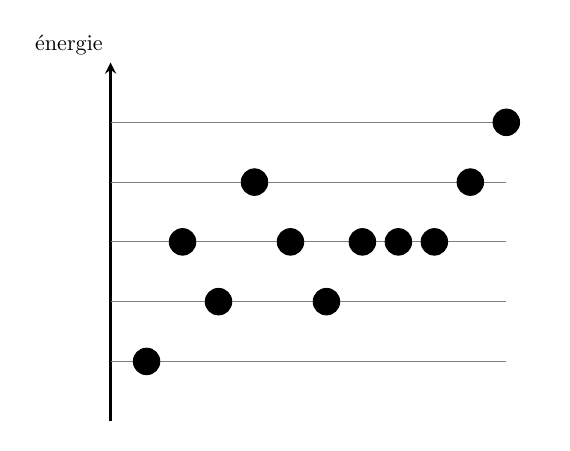
\begin{tikzpicture}[scale=0.8]
\begin{axis}[axis lines=left,
y axis line style={very thick},
x axis line style={draw=none},
ylabel={énergie},
xmin=0,xmax=12,
ymin=0,ymax=6,
xmajorticks=false,
ymajorticks=false,
xlabel style={at={(axis description cs:1,0)},anchor=north west},
ylabel style={at={(axis description cs:0,1)},anchor=south east,rotate=-90}]
\pgfplotsinvokeforeach{1,...,5}{\draw[gray] (0,#1) -- (11,#1);}
\filldraw (1,1) circle (6pt);
\filldraw (2,3) circle (6pt);
\filldraw (3,2) circle (6pt);
\filldraw (4,4) circle (6pt);
\filldraw (5,3) circle (6pt);
\filldraw (6,2) circle (6pt);
\filldraw (7,3) circle (6pt);
\filldraw (8,3) circle (6pt);
\filldraw (9,3) circle (6pt);
\filldraw (10,4) circle (6pt);
\filldraw (11,5) circle (6pt);
\end{axis}
\end{tikzpicture}
\hskip5pt
\begin{tikzpicture}[scale=0.8]
\begin{axis}[axis lines=left,
xlabel={nombre d'atomes},
ylabel={énergie},
xmin=0,xmax=12,
ymin=0,ymax=6,
xmajorticks=false,
ymajorticks=false,
xlabel style={at={(axis description cs:1,0)},anchor=south west},
ylabel style={at={(axis description cs:0,1)},anchor=south east,rotate=-90}]
\addplot[ultra thick,samples=1000] (exp(-(x-3)*(x-3))*8,x);
\draw[dashed] (0,3) -- (12,3);
\end{axis}
\end{tikzpicture}

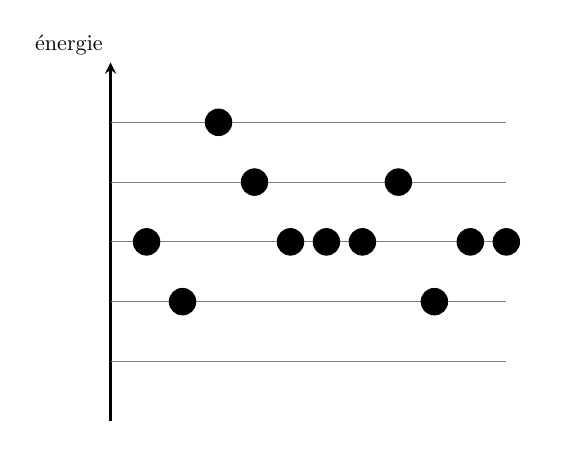
\begin{tikzpicture}[scale=0.8]
\begin{axis}[axis lines=left,
y axis line style={very thick},
x axis line style={draw=none},
ylabel={énergie},
xmin=0,xmax=12,
ymin=0,ymax=6,
xmajorticks=false,
ymajorticks=false,
xlabel style={at={(axis description cs:1,0)},anchor=north west},
ylabel style={at={(axis description cs:0,1)},anchor=south east,rotate=-90}]
\pgfplotsinvokeforeach{1,...,5}{\draw[gray] (0,#1) -- (11,#1);}
\filldraw (1,3) circle (6pt);
\filldraw (2,2) circle (6pt);
\filldraw (3,5) circle (6pt);
\filldraw (4,4) circle (6pt);
\filldraw (5,3) circle (6pt);
\filldraw (6,3) circle (6pt);
\filldraw (7,3) circle (6pt);
\filldraw (8,4) circle (6pt);
\filldraw (9,2) circle (6pt);
\filldraw (10,3) circle (6pt);
\filldraw (11,3) circle (6pt);
\end{axis}
\end{tikzpicture}
\hskip5pt
\begin{tikzpicture}[scale=0.8]
\begin{axis}[axis lines=left,
xlabel={nombre d'atomes},
ylabel={énergie},
xmin=0,xmax=12,
ymin=0,ymax=6,
xmajorticks=false,
ymajorticks=false,
xlabel style={at={(axis description cs:1,0)},anchor=south west},
ylabel style={at={(axis description cs:0,1)},anchor=south east,rotate=-90}]
\addplot[ultra thick,samples=1000] (exp(-(x-3)*(x-3))*8,x);
\draw[dashed] (0,3) -- (12,3);
\end{axis}
\end{tikzpicture}

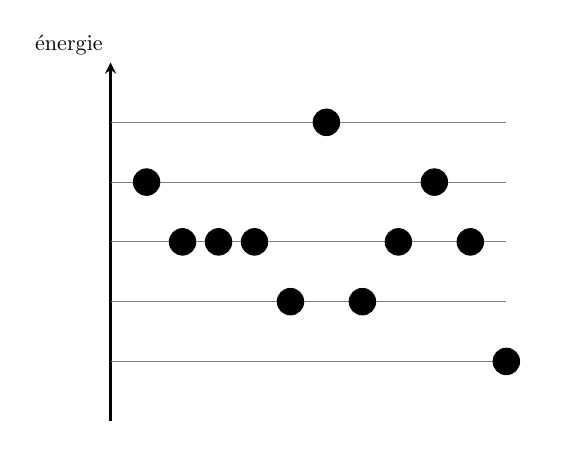
\begin{tikzpicture}[scale=0.8]
\begin{axis}[axis lines=left,
y axis line style={very thick},
x axis line style={draw=none},
ylabel={énergie},
xmin=0,xmax=12,
ymin=0,ymax=6,
xmajorticks=false,
ymajorticks=false,
xlabel style={at={(axis description cs:1,0)},anchor=north west},
ylabel style={at={(axis description cs:0,1)},anchor=south east,rotate=-90}]
\pgfplotsinvokeforeach{1,...,5}{\draw[gray] (0,#1) -- (11,#1);}
\filldraw (1,4) circle (6pt);
\filldraw (2,3) circle (6pt);
\filldraw (3,3) circle (6pt);
\filldraw (4,3) circle (6pt);
\filldraw (5,2) circle (6pt);
\filldraw (6,5) circle (6pt);
\filldraw (7,2) circle (6pt);
\filldraw (8,3) circle (6pt);
\filldraw (9,4) circle (6pt);
\filldraw (10,3) circle (6pt);
\filldraw (11,1) circle (6pt);
\end{axis}
\end{tikzpicture}
\hskip5pt
\begin{tikzpicture}[scale=0.8]
\begin{axis}[axis lines=left,
xlabel={nombre d'atomes},
ylabel={énergie},
xmin=0,xmax=12,
ymin=0,ymax=6,
xmajorticks=false,
ymajorticks=false,
xlabel style={at={(axis description cs:1,0)},anchor=south west},
ylabel style={at={(axis description cs:0,1)},anchor=south east,rotate=-90}]
\addplot[ultra thick,samples=1000] (exp(-(x-3)*(x-3))*8,x);
\draw[dashed] (0,3) -- (12,3);
\end{axis}
\end{tikzpicture}

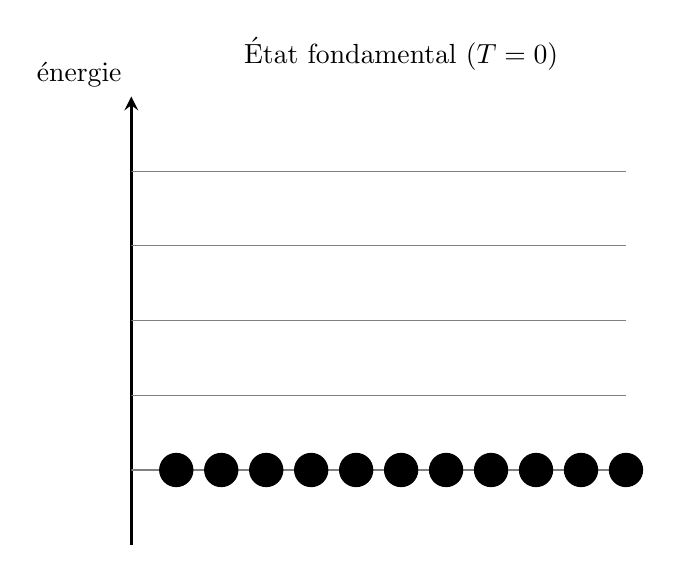
\begin{tikzpicture}
\begin{axis}[axis lines=left,
title={État fondamental (\(T=\SI{0}{\kelvin}\))},
y axis line style={very thick},
x axis line style={draw=none},
ylabel={énergie},
xmin=0,xmax=12,
ymin=0,ymax=6,
xmajorticks=false,
ymajorticks=false,
xlabel style={at={(axis description cs:1,0)},anchor=north west},
ylabel style={at={(axis description cs:0,1)},anchor=south east,rotate=-90}]
\pgfplotsinvokeforeach{1,...,5}{\draw[gray] (0,#1) -- (11,#1);}
\filldraw (1,1) circle (6pt);
\filldraw (2,1) circle (6pt);
\filldraw (3,1) circle (6pt);
\filldraw (4,1) circle (6pt);
\filldraw (5,1) circle (6pt);
\filldraw (6,1) circle (6pt);
\filldraw (7,1) circle (6pt);
\filldraw (8,1) circle (6pt);
\filldraw (9,1) circle (6pt);
\filldraw (10,1) circle (6pt);
\filldraw (11,1) circle (6pt);
\end{axis}
\end{tikzpicture}
\end{center}

À la température du zéro absolu, tous les atomes sont dans leur état de plus basse énergie. Dès que la température s'élève, les atomes s'écartent de cet état fondamental : à un température donnée, leur agitation thermique moyenne peut résulter d'un grand nombre de configurations différentes à l'échelle atomique (trois sont représentées ici).

\subsubsection{Quelle est l'étendue des valeurs que peut prendre la température ?}

Les \(\SI{300}{\kelvin}\) qui règnent sur Terre laissent l'eau s'écouler en rivière, jaillir en cascades. C'est la condition préalable à l'émergence de la vie sur la planète. Cette température clémente règne-t-elle ailleurs dans l'Univers ? Nul ne le sait aujourd'hui, mais les plus extrêmes s'y côtoient : le gaz qui est en passe d'être englouti par les astres les plus denses, trous noirs ou étoiles à neutrons, affiche une température de plus d'un million de degrés. Ainsi chauffée, la matière se transforme en plasma : les électrons se libèrent du giron de l'atome, et le noyau part en solitaire. Un véritable océan d'électrons et de noyaux atomiques à la dérive. Or, cet état de la matière est extrêmement courant dans l'Univers : ce gaz chaud émet des rayons très énergétiques, des X et des gamma, que l'on peut capter grâce aux satellites d'observations astronomiques.

Mais les températures à proximité d'un trou noir sont sans commune mesure avec celles qui font le quotidien des théoriciens. Les cosmologistes qui tentent d'expliquer à coup d'équations les premiers instants de l'Univers ont estimé la température qui colle à leurs modèles : ainsi après un milliardième de seconde après le Big Bang, aurait régné une température de \(\SI{e13}{\kelvin}\), indispensable pour la formation des premières particules stables, les protons et les neutrons, éléments des futurs noyaux atomiques...

Côté basses températures, la nature se fait largement doubler par les expériences de laboratoire : des solides entiers ont pu être refroidis jusqu'à quelques millionièmes de Kelvin, tandis que les atomes froids frisent quelques milliardièmes de Kelvin. Qu'est-ce qui distingue un atome froid de son cousin réchauffé ? L'atome glacé reste comme suspendu dans le vide, sans cette agitation thermique qui distingue son état habituel lorsqu'il est enfoui au sein d'un objet à température ambiante. Pour le tenir ainsi, on braque sur sa personne une multitude de lasers d'égale intensité. Quant à l'intérêt de l'opération... ce n'est pas de voir son nom gravé dans le livre des records, mais de manipuler les atomes quasiment comme des prunes : les déplacer un par un et les compter. Dans quel but ? Celui de vérifier les lois de la physique quantique, et, à plus long terme, de fabriquer des faisceaux laser où les grains de lumière seront remplacés par les atomes.

\subsubsection{Quelle gamme de températures convient à la vie ?}

Aux températures élevées, la matière a la faculté -- en fournissant de l'énergie interne sous forme de chaleur -- d'arracher un électron à un atome et ainsi de l'ioniser. Or, il s'agit là du principe même de la réactivité chimique. La température impose la vitesse des réactions chimiques : oxydation, digestion, putréfaction, tout ce qui relève de la chimie lui doit une fière chandelle. Sans oublier la vie qui englobe une multitude de réactions : le métabolisme du vivant n'est possible que dans une gamme restreinte de températures. Si les \(\SI{37}{\degreeCelsius}\) du corps humain optimisent la vitesse des réactions chimiques, c'est en grande partie à cause de l'existence de l'eau sous sa forme liquide. C'est elle qui se charge, par le biais des fluides biologiques, de transporter et de distribuer les substances nécessaires aux différents organes. La vie est-elle possible sans eau liquide ? Jamais vu, jamais envisagé, répondent en chœur les exobiologistes. Mais des cas d'adaptation aux températures extrêmes sont suivis de très près. Côté forte température, le record du vivant dépasse la centaine de degrés : à proximité des sources hydrothermales des grands fonds, dans une eau à plus de \(\SI{100}{\degreeCelsius}\) où pullulent des colonies de micro-organismes...

À l'autre bout de l'échelle, les psychrophiles sont des organismes unicellulaires qui se contentent d'un petit \(\SI{20}{\degreeCelsius}\), voire moins. Certains restent en vie à des températures de \(\SI{-12}{\degreeCelsius}\). Non pas qu'ils se passent d'eau liquide, vivant au ralenti, mais parce qu'ils ont la faculté de conserver l'eau sous forme liquide à des températures inférieures au point de congélation. Leur secret ? Le même que des milliards d'automobilistes pris par le froid hivernal : la cellule psychrophile produit des molécules antigel à base de sucre et d'alcool.

L'antigel est aussi la substance fétiche de certaines personnes qui, séduites par la cryogénisation, ont émis le désir de se réveiller un jour dans un monde meilleur : après leur mort, les fluides vitaux de leurs corps ont été remplacés par... du glycérol... qui est censé préserver leur dépouille dans un état de conservation telle que, des années plus tard, les progrès de la science aidant, ils puissent revenir à la vie. L'escroquerie a rencontré quelque succès outre-Atlantique. De leur côté, les cryobiologistes ont déjà réussi la conservation de cellules : les banques de sang et de sperme utilisent des méthodes de conservation par le froid. Mais leur objectif pour les prochaines décennies est de concevoir une banque d'organes : des reins, foies ou poumons à prélever, à conserver et au besoin à transplanter, parfois bien longtemps après. La difficulté dans ce domaine est de refroidir très rapidement -- vitrifier, car la même technique est utilisée pour produire des verres --, afin que les cristaux de glace ne puissent pas se former. En effet, l'eau en gelant voit son volume augmenter et ferait éclater les membranes. De plus, la glace en se constituant abandonne ses sels minéraux. L'antigel idéal se laisse encore désirer.

\subsubsection{Pourquoi tenter d'atteindre de très basses températures ?}

Pour démasquer la vraie nature de la matière : la température, à cause de l'agitation qu'elle provoque chez les atomes, cache quelques phénomènes fondamentaux dont la compréhension éclairerait tout un pan de la physique. La supraconductivité, par exemple, en fait partie : il s'agit de la faculté de transporter du courant sans perte. En dessous d'une certaine température critique, la résistivité électrique du matériau devient pratiquement nulle, il devient alors supraconducteur. Seulement les matériaux disponibles ont des températures critiques si basses qu'aujourd'hui le gain d'énergie ne rembourserait pas le coût du refroidissement. Du coup, l'utilisation des supraconducteurs est pour l'instant limitée aux instruments de mesure des très faibles champs magnétiques, aux outils de diagnostic médical fonctionnant sur la base de la résonance magnétique nucléaire, ou encore au sein de gros accélérateurs de particules.

Une autre propriété de la matière est à mettre en parallèle avec la supraconductivité : elle se manifeste chez l'hélium 4 liquide. Placé dans un récipient, celui-ci grimpe aux parois pour se déverser spontanément. En effet, en dessous d'une certaine température critique, l'hélium 4 perd toute viscosité : il se transforme en un fluide parfait qui n'oppose aucune adhérence aux parois. Ces deux bizarreries qui se manifestent à basse température sont encore dans l'attente d'une théorie qui rende compte de tous leurs aspects.